
\documentclass{beamer}

\usepackage{algpseudocode, color, colortbl}

\usepackage{hyperref}
\hypersetup{
    colorlinks=true,
    urlcolor=blue,
}

\usetheme{Montpellier}
\usecolortheme{rose}

% page numbers, from
% https://tex.stackexchange.com/questions/137022/how-to-insert-page-number-in-beamer-navigation-symbols
\expandafter\def\expandafter\insertshorttitle\expandafter{%
  \insertshorttitle\hfill%
  \insertframenumber\,/\,\inserttotalframenumber}

\definecolor{Gray}{gray}{0.8}
\newcolumntype{g}{>{\columncolor{Gray}}c}

\newcommand{\stanza}{ \\~\ }

\title{07. Amortized Analysis and Fibonacci Heaps}
\subtitle{CPSC 535 $\sim$ Spring 2019}
\author{Kevin A. Wortman}
\institute{ 
\includegraphics[height=2cm]{csuf-logo-cmyk} }
\date{March 11, 2019 \stanza

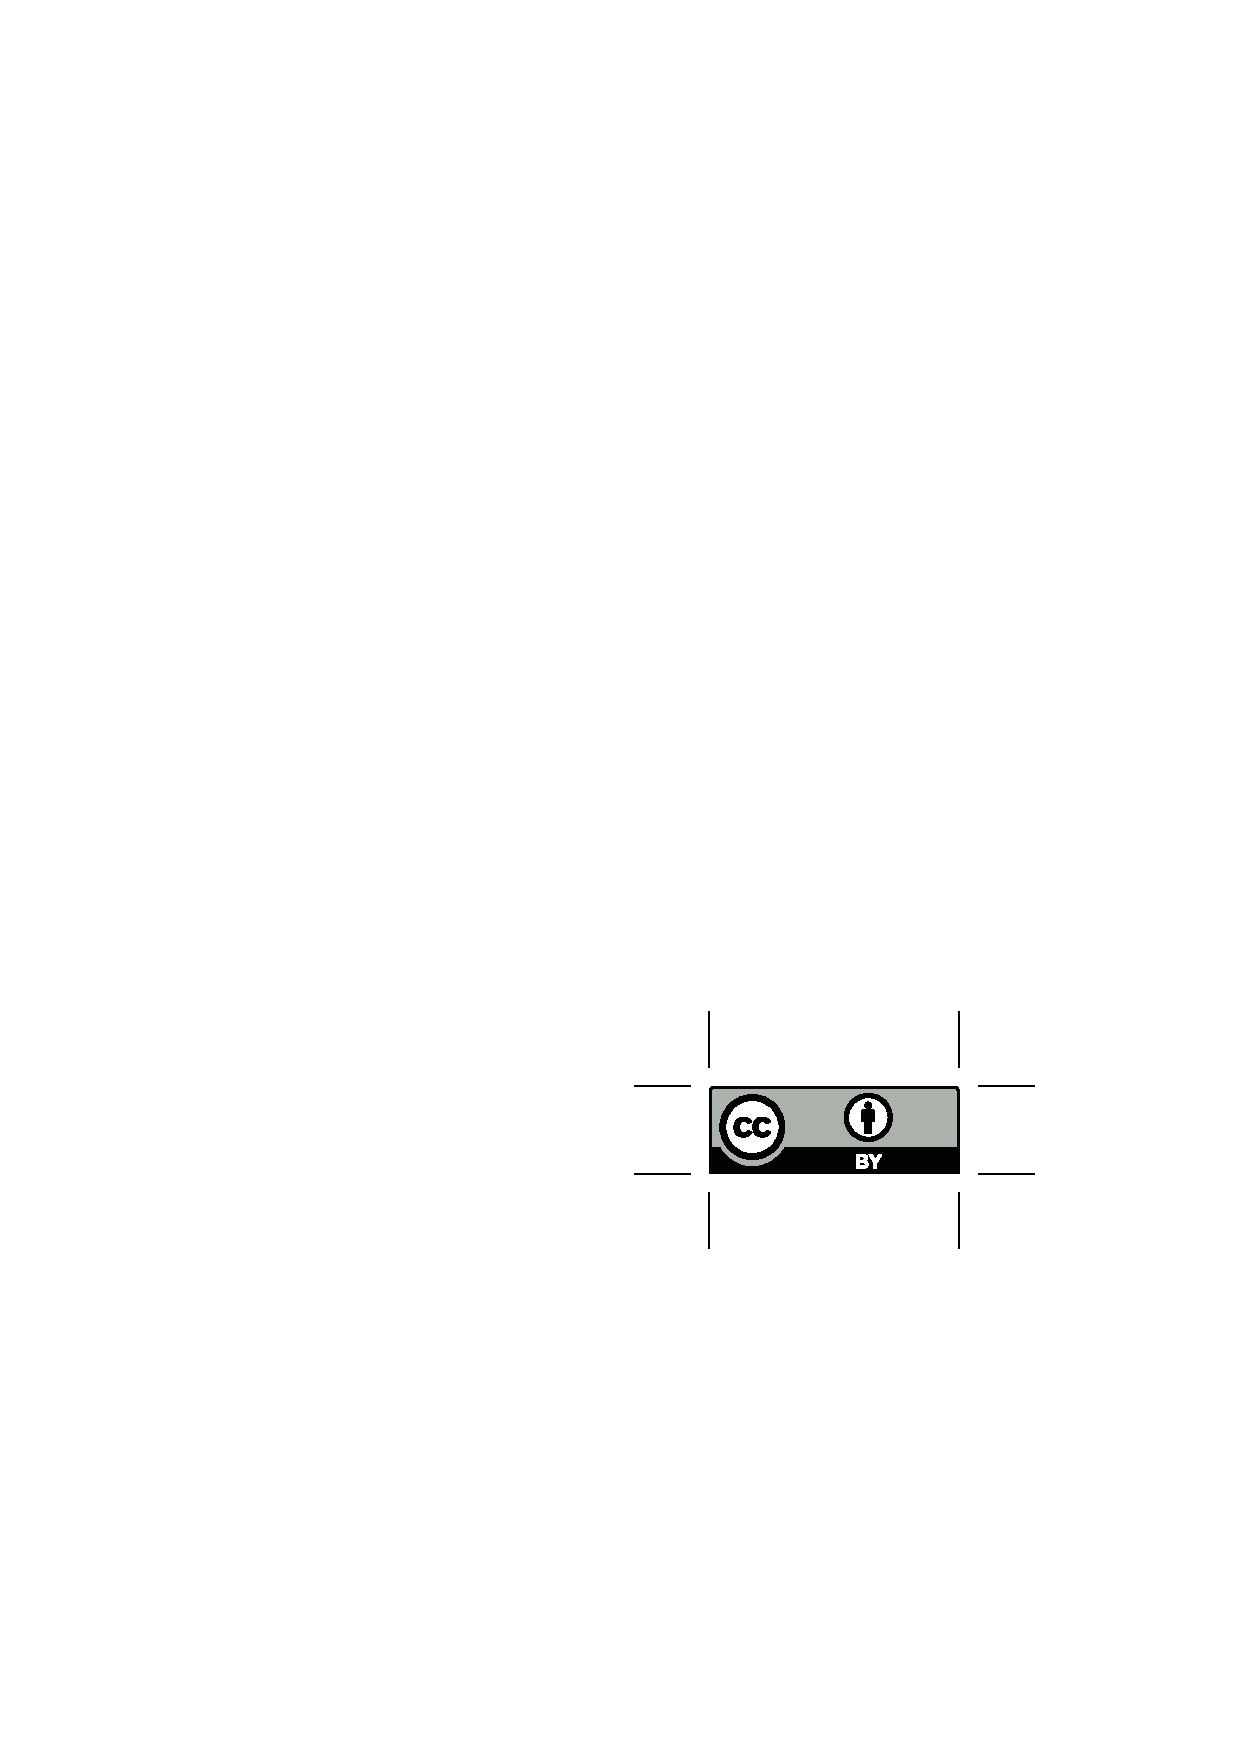
\includegraphics[height=14pt]{by} \\

{\tiny
This work is licensed under a
\href{http://creativecommons.org/licenses/by/4.0/}{Creative Commons Attribution 4.0 International License}.
}}

\begin{document}

\begin{frame}
  \titlepage
\end{frame}

\begin{frame} \frametitle{Amortized Efficiency}
\textbf{amortized} performance
\begin{itemize}
  \item \emph{amortized efficiency:} average of worst-case time over any sequence of operations
  \item different from (probabalistic) expected efficiency, which is averaged over random choices
    made by a PRNG
  \item amortized time bound is a weaker math condition than the same
    worst-case bound
  \item e.g. $\Theta(1)$ amortized vs. $\Theta(1)$ worst-case
  \item $\implies$ downgrading to an amortized bound may admit upgrades to
    other aspects of a data structure
\end{itemize}
\end{frame}

\begin{frame} \frametitle{Big Idea in Algorithm Design: Work Smart not Hard}
Lifecycle of an implemented algorithm:
\begin{center}
  \begin{tabular}{ll}
    \textbf{Phase of Life} & \textbf{Frequency of Creation} \\
    design and analysis & once, by discoverer and peer reviewers \\
    learned by students & annually, by thousands \\
    implemented & once per programming language lifetime (decade) \\
    run and maintained & millions-billions of times indefinitely \\
  \end{tabular}
\end{center}
\begin{itemize}
\item given the choice, we'd prefer for the ongoing tasks to be easy
\item even if that means the one-time phases are complicated
\item holy grail: algorithm is tough to conceive and analyze, but easy to
  understand and implement
\item example: universal hashing, open addressing
\end{itemize}
\end{frame}

\begin{frame} \frametitle{Amortized Analysis --- What to Prove}
A \emph{splay tree} is a kind of binary search tree. \stanza

Lemma: the $INSERT, SEARCH,$ and $DELETE$ operations each take $\Theta(\log n)$
amortized time on a splay tree. \stanza

Would need to prove:
\begin{itemize}
  \item average time/operation $= \Theta(\log n)$
  \item or, any sequence of $n$ of these operations takes a grand total of
    $n \cdot \Theta(\log n) = \Theta(n \log n)$ worst-case time
  \item \underline{any} sequence: includes the worst-case for the data structure
  \item three conventional proof techniques
\end{itemize}
\end{frame}

\begin{frame} \frametitle{Aggregate Analysis}
\begin{itemize}
  \item count total time $T(n)$ for any sequence of $n$ operations
  \item $\implies$ each operation takes $T(n)/n$ amortized time
  \item pro: simple logic; from first principles
  \item con: only works when the goal is to prove all operations take the
    same time (e.g. $INSERT, SEARCH,$ and $DELETE$ are each $\Theta(\log n)$);
    wouldn't work if one of them is $\Theta(1)$
  \item con: not much inspiration for difficult analyses
\end{itemize}
\end{frame}

\begin{frame} \frametitle{The Accounting Method}
\begin{itemize}
  \item inspired by financial amortization, balanced budgets
  \item analyst picks a \textbf{cost} for each operation
    (ex.: $INSERT$ costs $4 \cdot \lceil \log_2 n \rceil$ units)
  \item some operations \textbf{over-charge} and turn a \textbf{profit} that is
    deposited somewhere in the structure (e.g. in a node)
  \item other operations \textbf{under-charge} and incur a \textbf{loss} that
    is withdrawn from prior deposits
  \item show: never go bankrupt, i.e. withdrawn units always exist
  \item show: for every operation,
    \[ \text{(charge)} + \text{(withdrawal)} \leq \text{actual time spent} \]
  \item $\implies \text{amortized time} = \text{charged cost}$
\end{itemize}
\end{frame}

\begin{frame} \frametitle{Accounting Method Pros/Cons}
  \begin{itemize}
    \item pro: possible to prove different amortized efficiency classes for
      each operation (e.g. one is $\Theta(1)$, another $\Theta(\log n)$)
    \item pro: cost story helps us reason through analysis
    \item loss operation $ = $ procrastinating, deferring work to later
    \item profit operation $ = $ catching up on deferred work
    \item con: cost story may overcomplicate things
    \item con: sometimes awkard to store profits in specific data structure
      locations
  \end{itemize}
\end{frame}

\begin{frame} \frametitle{Potential Method}
\begin{itemize}
  \item premise: for data structure $D,$ \textbf{potential function} $\Phi(D)$
  \item ($\Phi$ pronounced like ``fee'')
  \item potential is stored energy, like a battery
  \item amortized time of operation $=$ actual time $+$ change to $\Phi(D)$
  \item procrastinating/loss operations decrease $\Phi(D)$
  \item catch-up/profit operations increase $\Phi(D)$
  \item show: $\Phi(D) \geq 0$ always
  \item ultimately a less structured way of thinking of the accounting method
\end{itemize}
\end{frame}

\begin{frame} \frametitle{Fibonacci Heap Overview}
\begin{itemize}
  \item alternative to a binary heap (as in heapsort)
  \item pro: faster INSERT and DECREASE-KEY operations (optimal in fact)
  \item pro: supports additional operations
  \item con: more complicated to describe, implement, \emph{especially} analyze
  \item con: operations have amortized time bounds
  \item con: much worse constant factors, not in-place
  \item not currently practical
\end{itemize}
\end{frame}

\begin{frame} \frametitle{Mergeable Heap API}
CREATE-HEAP(): initialize empty heap \\
INSERT($H, x$): insert entry $x$ into $H$ \\
MINIMUM($H$): return minimum-key entry \\
EXTRACT-MIN($H$): remove and return minimum-key entry \\
UNION($H_1, H_2$): consume heaps $H_1, H_2$ and return a new heap with their elements \\
DECREASE-KEY($H, x, k)$: lower key of $x$ to $k$ \\
DELETE($H, x$): remove entry $x$ from $H$
\end{frame}

\begin{frame} \frametitle{Heap Efficiency Comparison}
  \begin{center}
    \begin{tabular}{lll}
      \textbf{Operation} & Binary Heap (worst-case) & Fib. Heap (amort.) \\ \hline
      CREATE-HEAP & $\Theta(1)$ & $\Theta(1)$ \\
      INSERT & $\Theta(\log n)$ & $\Theta(1)$  \\
      MINIMUM & $\Theta(1)$ & $\Theta(1)$ \\
      EXTRACT-MIN &  $\Theta(\log n)$ & $O(\log n)$ \\
      UNION & $\Theta(n)$ & $\Theta(1)$ \\
      DECREASE-KEY & $\Theta(\log n)$ & $\Theta(1)$ \\
      DELETE & $\Theta(\log n)$ & $\Theta(\log n)$
    \end{tabular}
  \end{center}
\end{frame}

\begin{frame} \frametitle{Fibonacci Heap Structure}
Overall heap $H$ has
\begin{itemize}
  \item a \emph{forest} of individual $k$-ary trees (nonbinary); each tree in min-heap-order
  \item $H.min$ = pointer to the root with the global minimum key
  \item $H.n$ = number of entries in heap
\end{itemize}

Each node $x$ has
\begin{itemize}
  \item $x.parent$ = parent node (NIL if root)
  \item $x.child$ = pointer to an arbitrary child
  \item $x.left, x.right$ = pointers to siblings
  \item (siblings are in circular, unsorted, doubly-linked lists)
  \item $x.degree$ = \# children
  \item $x.mark$ = boolean, true iff $x$ has lost a child since the last time
    $x$ was assigned a new parent (manages procrastination)
\end{itemize}
\end{frame}

\begin{frame} \frametitle{Potential Function and Degree Bound}
For analysis purposes, we define the potential function
\[ \Phi(H) = t(H) + 2 \cdot m(H) \]
where
\begin{itemize}
  \item $t(H) = $ \# trees in root list
  \item $m(H) = $ \# marked nodes
\end{itemize}

Claim: If Fibonacci heap $H$ has $n$ nodes, then the maximum degree (\# children) of any node,
written $D(n)$, is
\[ D(n) = O(\log n) .\]
\end{frame}

\begin{frame} \frametitle{CREATE-HEAP}
  \begin{algorithmic}[1]
    \Function{CREATE-HEAP}{}
    \State $H.min = $ NIL
    \State $H.n = 0$
    \State \Return{$H$}
    \EndFunction
  \end{algorithmic}
  \vspace{.5cm}
  Takes $\Theta(1)$ time; $t(H) = m(H) = 0$, so $\Phi(H) = 0$; no profit or loss.
\end{frame}

\begin{frame} \frametitle{INSERT Pseudocode}
Just create node, initialize node, insert into root list, update $H.min$ \stanza

{\small
\begin{algorithmic}[1]
  \Function{INSERT}{$H, x$}
  \State $x.degree = 0$
  \State $x.parent = x.child = $ NIL
  \State $x.mark = $ false
  \If{ $H.min == $ NIL }
    \State $H.min = x$
    \State $x.left = x.right = $ NIL
  \Else
    \State insert $x$ into root list as $H.min$'s right sibling
    \If{ $x.key < H.min.key$ }
      \State $H.min = x$
    \EndIf
  \EndIf
  \State $H.n++$
  \EndFunction
\end{algorithmic}
}
\end{frame}

\begin{frame} \frametitle{INSERT Analysis}
Actual time steps are $\Theta(1).$

Let $H$ be heap before INSERT, and $H'$ after; then \stanza

$t(H') = t(H) + 1$ (one tree created) \\
$m(H') = m(H)$ (no marking) \\
$\implies \Phi(H') = \Phi(H) + 1$ \stanza

$\therefore$ INSERT takes $O(1)+1 = O(1)$ amortized time.
\end{frame}

\begin{frame} \frametitle{MINIMUM}
Just follow the $H.min$ pointer. \stanza

$O(1)$ actual time. \stanza

No new trees, no new marked nodes, so $O(1)$ amortized time.
\end{frame}

\begin{frame} \frametitle{UNION}
  {\small
  \begin{algorithmic}[1]
    \Function{UNION}{$H_1, H_2$}
    \If{$H_1.n$ == 0}
      \State \Return{$H_2$}
    \ElsIf{$H_2.n$ == 0}
      \State \Return{$H_1$}
    \Else
      \State $H$ = new heap object
      \State $H.min = min(H_1.min, H_2.min)$
      \State $H.n = H_1.n + H_2.n$
      \State concatenate root lists of $H_1, H_2$ into one linked list
      \State \Return{$H$}
    \EndIf
    \EndFunction
  \end{algorithmic}
  }
  \vspace{.5cm}
  $O(1)$ actual time; trees and marked nodes move around, but their number
  is unchanged, so no change to $\Phi$; $O(1)$ amortized time.
\end{frame}

\begin{frame} \frametitle{So Far So Good}
So far all operations have been simple, and either potential-neutral
(CREATE-HEAP, MINIMUM), or increased potential (INSERT) \stanza

Indeed, $n$ INSERTs creates a glorified $n$-element linked list. \stanza

$\therefore$ need to expect remaining operations to be more complicated,
decrease potential, decrease length of root list.
\end{frame}

\begin{frame} \frametitle{EXTRACT-MIN}
Follow $H.min$ pointer; promote all children to roots; remove from root list;
CONSOLIDATE to shorten root list and find new $H.min.$

{\small
\begin{algorithmic}[1]
  \Function{EXTRACT-MIN}{$H$}
  \State $z = H.min$
  \For{each child $c$ of $z$}
    \State insert $c$ into $H$'s root list
    \State $c.parent = $ NIL
  \EndFor
  \State delete $z$ from root list
  \If{$H.n$ == 1}
    \State $H.min = NIL$ \Comment{heap just became empty}
  \Else
    \State CONSOLIDATE($H$) \Comment{compact root list, recompute $H.min$}
  \EndIf
  \State $H.n--$
  \State \Return{$z$}
  \EndFunction
\end{algorithmic}
}
\end{frame}

\begin{frame} \frametitle{Zooming in to CONSOLIDATE}
Before moving on, observe EXTRACT-MIN takes, aside from CONSOLIDATE,
$\Theta(\text{degree}(H.min))$ time; claimed this is $\Theta(\log n)$
\stanza

Contract for CONSOLIDATE: \stanza

\begin{algorithmic}[1]
  \Function{CONSOLIDATE}{$H$}
  \Require {$H.min$ invalid and $H.n$ == \#nodes + 1}
  \Ensure {$H.min$ valid and \#trees $\in O(\log n)$}
  \EndFunction
\end{algorithmic}
\end{frame}

\begin{frame} \frametitle{CONSOLIDATE Pseudocode}
  \begin{algorithmic}[1]
    \Function{CONSOLIDATE}{$H$}
    \State $A$ = UNIQUE-DEGREE-ARRAY($H$)
    \State ARRAY-TO-ROOT-LIST($H, A$)
    \State free $A$
    \State RECOMPUTE-MIN($H$)
    \EndFunction
  \end{algorithmic}
  \vspace{.5cm}
  Clearly $\Theta(1)$ time except for the three subroutines.
\end{frame}

\begin{frame} \frametitle{UNIQUE-DEGREE-ARRAY Pseudocode}
  {\small
  \begin{algorithmic}[1]
    \Function{UNIQUE-DEGREE-ARRAY}{$H$}
    \Ensure { returns $A[0..D(H.n)]$ where $A[d]$ = only root w/ degree $d$ }
    \State $A[0..D(H.n)] = $ new array of node pointers, all NIL
    \For { each root node $r$ in $H$ } \Comment{move $r$ into $A$}
      \State $p = r$ \Comment{parent node that needs to move into $A$}
      \While { $A[p.degree] \ne $ NIL } \Comment{another node in the way}
        \State $c = A[p.degree]$ \Comment{$p, c$ have same degree}
        \State $A[p.degree] = $ NIL \Comment{we will link them into one tree}
        \If { $p.key > c.key$ }
          \State swap($p, c$) \Comment{ensure $c$ should be $p$'s child}
        \EndIf
        \State make $c$ a child of $p$, incrementing $p.degree$
        \State $c.mark = $ false
      \EndWhile
    \EndFor
    \State \Return{ $A$ }
    \EndFunction
  \end{algorithmic}
  }
\end{frame}

\begin{frame} \frametitle{UNIQUE-DEGREE-ARRAY Analysis}
  Create $A$: $O(D(n))$ time \stanza

  \textbf{for} loop --- aggregate analysis
  \begin{itemize}
    \item \# iterations = length of root list before CONSOLIDATE = $t(H) + D(n) - 1$
    \item each iteration of inner \textbf{while} loop links two roots into one, decrementing \# roots
    \item \# roots at end of CONSOLIDATE $\leq $ size of $A = D(n)+1$
    \item $\implies$ total time in all \textbf{while} iterations is
    \[ \big(t(H)+D(n)-1 \big) - \big( D(n) + 1 \big) = t(H) - 2 \]
    \item $\implies$ total time in \textbf{for} loop is
    \[ \big(t(H) + D(n) - 1\big) + \big(t(H)-2 \big) \leq 2 \cdot t(H) + D(n) \]
  \end{itemize}

  total for UNIQUE-DEGREE-ARRAY is $O(t(H) + D(n))$
\end{frame}

\begin{frame} \frametitle{ARRAY-TO-ROOT-LIST}
  \begin{algorithmic}[1]
    \Function{ARRAY-TO-ROOT-LIST}{$H, A$}
    \State clear $H$'s root list to empty
    \For { index $i$ of $A$ }
      \If { $A[i] \ne $ NIL }
        \State insert $A[i]$ into $H$'s root list
      \EndIf
    \EndFor
    \EndFunction
  \end{algorithmic}
  \vspace{.5cm}
  $O(D(n))$ time
\end{frame}

\begin{frame} \frametitle{RECOMPUTE-MIN}
  \begin{algorithmic}[1]
    \Function{RECOMPUTE-MIN}{$H$}
    \State $H.min = $ NIL
    \For { node $r$ in $H$'s root list }
      \If { $H.min$ == NIL }
        \State $H.min$ = $A[i]$
      \ElsIf { $H.min.key > r.key$ }
        \State $H.min = r$
      \EndIf
    \EndFor
    \EndFunction
  \end{algorithmic}
  \vspace{.5cm}
  $O(D(n))$ time
\end{frame}

\begin{frame} \frametitle{CONSOLIDATE Worst-Case Analysis}
  \begin{algorithmic}[1]
    \Function{CONSOLIDATE}{$H$}
    \State $A$ = UNIQUE-DEGREE-ARRAY($H$) \Comment{$O(D(n)+t(H))$}
    \State ARRAY-TO-ROOT-LIST($H, A$) \Comment{$O(D(n)))$}
    \State free $A$ \Comment{$O(1)$}
    \State RECOMPUTE-MIN($H$) \Comment{$O(D(n))$}
    \EndFunction
  \end{algorithmic}
  \vspace{.5cm}
  Time spent is
  \[ O(D(n) + t(H) + D(n) + 1 + D(n)) = O(3 \cdot D(n) + t(H)) = O(\log n + t(H)) . \]
  Want this to be $O(\log n)$; the $t(H)$ overage can be withdrawn from the
  potential function.
\end{frame}

\begin{frame} \frametitle{CONSOLIDATE Amortized Analysis}
Recall potential function
\[ \Phi(H) = t(H) + 2 \cdot m(H) \]
Let $H'$ be $H$ after EXTRACT-MIN \\
EXTRACT-MIN does not mark any nodes, so $m(H') = m(H).$ \\
\# roots decreases: $t(H') = D(n)+1 \leq t(H)$
\[ \Phi(H') = t(H') + 2 \cdot m(H') = \big(D(n)+1\big) + 2 \cdot m(H) \]
\[ \Phi(H) - \Phi(H') = t(H) - \big(D(n)+1\big) \]
Amortized cost of EXTRACT-MIN
\[ = \Delta\Phi = O(t(H) + D(n)) - O(t(H) - D(n) - 1) = O(2\cdot D(n)) = O(\log n) \]
\end{frame}

\begin{frame} \frametitle{Where did that time come from? Accounting Perspective}
\begin{itemize}
  \item potential function's $t(H)$ term over-charges INSERT and under-charges EXTRACT-MIN
  \item when $t(H) = O(\log n)$, EXTRACT-MIN takes $O(\log n)$ worst-case time
  \item first $\log n$ roots are ``clean'', remaining $t(H)-\log n$ are ``mess''
  \item deposit $O(1)$ time when INSERTing a messy root
  \item withdraw those deposits in CONSOLIDATE
  \item 1 deposit pays for making 1 messy root a child of a clean parent
  \item (recall that link operation takes $O(1)$ time)
  \item hard to use accounting method directly because the identity of the clean
    nodes changes during CONSOLIDATE based on heap-order
\end{itemize}
\end{frame}

\begin{frame} \frametitle{DELETE}
  \begin{algorithmic}[1]
    \Function{DELETE}{$H, x$}
    \State DECREASE-KEY($H, x, -\infty$)
    \State EXTRACT-MIN($H$)
    \EndFunction
  \end{algorithmic}
\vspace{.5cm}
Know EXTRACT-MIN is $O(\log n)$ amortized time. \stanza

Claim: DECREASE-KEY is $O(1)$ amortized time. \stanza

$\implies$ DELETE is $O(\log n)$ amortized time.
\end{frame}

\begin{frame} \frametitle{DECREASE-KEY Sketch}
DECREASE-KEY($H, x, k$)
\begin{itemize}
  \item update $x.key = k$
  \item if $x$ is a root, or heap-order maintained, done
  \item else \textbf{cut} $x$
    \begin{itemize}
      \item make $x$ a root, no longer a child of parent $p$
      \item update $H.min$ if $x$ is new minimum
      \item mark $p$; but if $p$ was already marked, recursively cut $p$
    \end{itemize}
  \item $O(1)$ time not counting recursive cuts
  \item recursive cuts are paid for by withdrawing potential
\end{itemize}
\end{frame}

\begin{frame} \frametitle{Heap Efficiency Comparison}
  \begin{center}
    \begin{tabular}{lll}
      \textbf{Operation} & Binary Heap (worst-case) & Fib. Heap (amort.) \\ \hline
      CREATE-HEAP & $\Theta(1)$ & $\Theta(1)$ \\
      INSERT & $\Theta(\log n)$ & $\Theta(1)$  \\
      MINIMUM & $\Theta(1)$ & $\Theta(1)$ \\
      EXTRACT-MIN &  $\Theta(\log n)$ & $O(\log n)$ \\
      UNION & $\Theta(n)$ & $\Theta(1)$ \\
      DECREASE-KEY & $\Theta(\log n)$ & $\Theta(1)$ \\
      DELETE & $\Theta(\log n)$ & $\Theta(\log n)$
    \end{tabular}
  \end{center}
\end{frame}

\end{document}
